\begin{center}
    \textbf{--------- Lezione 6 - 12 ottobre 2020 ---------}
\end{center}

\section{Progettazione delle interfacce}
Mentre per i dispositivi tradizionali abbiamo come dispositivi di input tastiere, mouse, microfono ecc. per i dispositivi mobili abbiamo touch screen, pulsanti fisici e altri sensori come accelerometro, giroscopi. 

Il touch screen permette l'interazione molto più sofisticata del mouse, infatti è possibile definire gesture più complesse. 
Ci sono dei casi in cui introdurre dei gesti può risaltare a pieno le funzionalità di uno schermo touch come in un'applicazione per i non vedenti. 

Nei dispositivi tradizionali chi progetta le applicazioni, progetta una sola interfaccia, nei dispositivi mobili invece le dimensioni variano e bisogna progettare un'interfaccia diversa. 

L'orientamento può cambiare con l'orientamento del dispositivo e quindi la GUI si deve adattare. 

Ci sono diversi problemi: 
\begin{itemize}
    \item la risoluzione: se la definizione aumenta (cioè aumenta il numero di pixel per pollice) gli oggetti di interfaccia potrebbero essere troppo piccoli
    \item la grandezza di uno schermo: su schermi con risoluzioni diverse gli oggetti potrebbero avere posizioni poche estetiche (es: occupare solo la parte sinistra dello schermo) o non funzionali (es: elementi che non sono visibili)
\end{itemize}

\subsection{Responsive design}
L'idea del responsive design è di progettare interfacce per schermi con risoluzione diverse. 
Il responsive design nasce per il web, ma molte soluzioni sono state adottate per le applicazioni per dispositivi mobili.
Il responsive design fa affidamento su funzionalità (di tool, librerie, ecc.) che lo rendono possibile. 

Gli strumenti principali della progettazione responsive sono:
\begin{itemize}
    \item i layout "liquidi"
    \item Ri-definizione delle schermate
    \item densità di pixel
\end{itemize}

\subsubsection{I layout "liquidi" (o "fluidi")}
Non vogliamo definire delle dimensioni assolute nei layout, ma vogliamo usare delle dimensioni relative ad altri elementi, come alla dimensione dello schermo, allo spazio reso disponibile dal "contenitore" oppure allo spazio richiesto dal contenuto.
Degli esempi ne sono:
\begin{itemize}
    \item android:layout\_width:"match\_parent" \\
          android:layout\_height:"wrap\_content"
    \item bootstrap: è una delle librerie più usate nello sviluppo web. Divide lo schermo in 12 colonne, quando specifichiamo la dimensione di un elemento, possiamo dire quanto deve essere largo in colonne. Ad esempio un pulsante può essere largo 3 colonne, significa che deve essere largo 1/4 della schermata e in questo modo si definisce la dimensione di un elemento in termini relativi, non assoluti
\end{itemize}

\subsubsection{Ri-definizione delle schermate}
I layout liquidi solitamente permettono di scrivere poco codice e sono un'ottima soluzione quando riescono a garantire una buona UX. 
A volte però non sono sufficienti perché su schermi diversi potrebbe essere necessario progettare interfacce utente totalmente differenti, a volte infatti si riprogetta l'intero schema di navigazione. 
\\ Non voglio rilasciare app diverse per ogni dispositivo, quindi tipicamente si usano strumenti che ci permettono di implementare interfacce diverse in funzione di vari parametri dello schermo. 

\subsubsection{Densità di pixel}
Gli informatici misurano le dimensioni degli oggetti sullo schermo 
in pixel, ma il problema è che maggiore è la definizione di uno schermo, minore la dimensione degli oggetti 
La soluzione è definire una dimensione che non cambia al variare delle densità di pixel sullo schermo: density independent pixel (dip o dp).
Il dp è un'unità di misura della lunghezza in mm che equivale ad un pixel con una densità di 160 dpi. Se la risoluzione raddoppia 1dp = 2dp. I dpi misurano il numero di pixel che ci sono in un inch: 2,54 cm. 160 dpi significa che in un pollice ci sono 160 pixel

\subsection{Navigazione}
Nelle applicazioni per dispositivi mobili in genere ogni schermata 
mostra un solo task e l'applicazione deve permettere di navigare tra diversi task.
Su dispositivi con schermi più grandi si possono progettare più task in un’unica schermata.

Lo schema di navigazione definisce come l'utente si muoverà tra le varie schermate. 
Non è necessario definire il dettaglio grafico di ogni schermata, basta indicare la funzionalità.
Le funzionalità più importanti/frequenti devono essere presentate il prima possibile all'utente.
La prima schermata mostrata all'utente può variare: primo avvio /
avvii successivi.

La navigazione si può organizzare in due modi diversi:
\begin{itemize}
    \item sequenziale: realizzata con una barra di navigazione in cui da una schermata mi sposto ad un'altra in sequenza (avanti o indietro)
    \begin{center}
        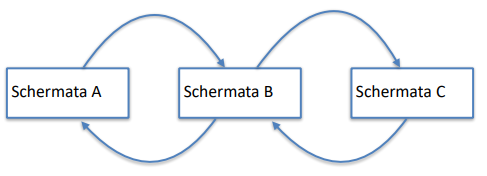
\includegraphics[width=.5\textwidth]{images/Mobile computing/6. Progettazione/navigazione sequenziale.PNG}
    \end{center}
    \item per task: permette di saltare da una schermata ad un'altra in modo diretto
    \begin{center}
        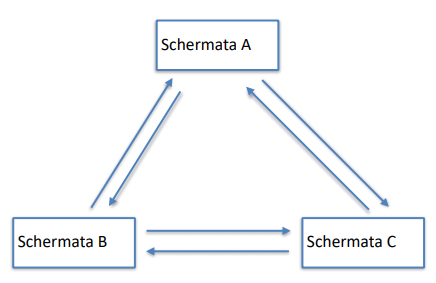
\includegraphics[width=.5\textwidth]{images/Mobile computing/6. Progettazione/navigazione per task.PNG}
    \end{center}
\end{itemize}

Una volta completato lo schema di navigazione bisogna progettare le 
singole schermate. A volte ci si rende conto che una schermata va divisa in due o più, oppure che due schermate si possono accorpare. In questo modo si torna a modificare lo schema di navigazione. Se ci rendiamo di aver commesso un errore, basta poco per correggerlo, se invece lo individuiamo in fase di implementazione, il costo sarà più elevato. 

Gli strumenti di interfaccia sono forniti dal framework come ad esempio pulsanti, caselle di testo, ma è anche possibile creare nuovi oggetti. 

\section{Progettare la struttura del codice}
Un progetto complesso è meglio suddividerlo in più componenti logiche, grazie alle quali è più semplice:
\begin{itemize}
    \item risolvere il problema adottando la stessa struttura già usata da altri in casi simili in precedenza
    \item distribuire il lavoro tra vari membri del team di lavoro
    \item valutare la correttezza delle singole componenti
    \item correggere eventuali errori
    \item mantenere il codice nel tempo: aggiornare le componenti ed il codice che dobbiamo aggiornare è più contenuto
\end{itemize}

Queste componenti logiche in alcuni casi possono corrispondere con componenti tecniche (es: una classe o un package) ma questo non è necessario. 

\subsection{I pattern di progettazione}
La progettazione della struttura del codice spetta al programmatore ed è specifica di un singolo progetto. 
I pattern di progettazione suggeriscono una possibile soluzione a problemi specifici nel codice o alla progettazione di massima della struttura del codice. 

\subsection{MVC: Model View Controller}
Nasce prima che nascono i dispositivi mobili e nasce per la progettazione di applicazioni con interfaccia grafica. 
È parte integrante dei framework ed è utilizzato in quasi tutte le applicazioni per dispositivi mobili.

L'idea è quella di dividere l'applicazione in tre componenti che vanno tenute nel modo più separato possibile:
\begin{itemize}
    \item Model: organizza e struttura i dati dell'applicazione. Definisce le operazioni sui dati ai quali le altre componenti possono accedere. Spesso si occupa di:
    \begin{itemize}
        \item creare oggetti dalla memoria persistente
        \item salvare gli oggetti nella memoria persistente
        \item serializzare e de-serializzare i dati
    \end{itemize}
    Ad esempio in un social network avremo un model che contiene il profilo
    \item View: presenta il contenuto all'utente. Le classi della view sono spesso fornite all'interno del framework dell'ambiente di sviluppo. Si possono usare degli oggetti già creati o possono essere personalizzati
    \item Controller: agisce come intermediario tra la View e la Model. Gestisce il ciclo di vita di un'applicazione e gestisce gli eventi
\end{itemize}

\begin{figure}[!ht]
    \centering
    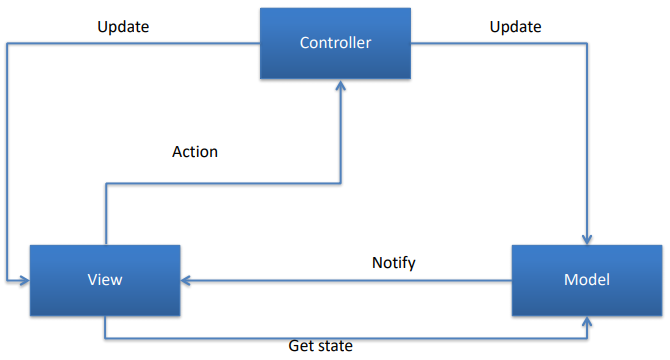
\includegraphics[width=.8\textwidth]{images/Mobile computing/6. Progettazione/struttura originale MVC.PNG}
    \caption{Struttura originale di MVC}
    \label{fig:MVC}
\end{figure}
La View notifica le azioni al Controller che può aggiornare o la View o la Model. Il Controller fa partire la richiesta. La Model quando riceve delle modifiche, può notificare la View che può leggere lo stato per aggiornarsi di conseguenza. 

Per i dispositivi mobili viene usato il Model View Presenter (MVP).
\newpage
\begin{figure}[!ht]
    \centering
    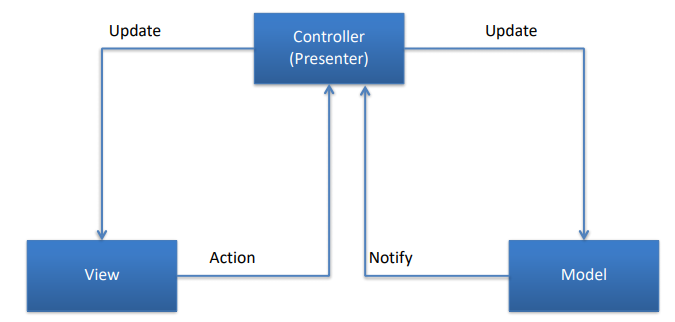
\includegraphics[width=.7\textwidth]{images/Mobile computing/6. Progettazione/MVP.PNG}
    \caption{Interpretazione Apple di MVP}
    \label{fig:MVP}
\end{figure}
La differenza con MVC è che Model e View non comunicano direttamente. Model notifica il Controller. La View notifica le azioni al Controller che può aggiornare View o Model. Se aggiorna la Model, questa può notificare al Controller che nel caso notifica la View. 

Uno dei pattern per separare le componenti è Observer. 

\subsection{Pattern Observer}
Ci sono oggetti "observer" che devono essere avvisati quando lo stato di un altro "subject" cambia. 
Lo stato può essere, ad esempio il valore di una o più variabili o un evento. 

Si implementa con tre componenti: 
\begin{itemize}
    \item una classe che rappresenta il subject
    \item una o più classi che rappresentano l'observer
    \item un'interfaccia (o classe astratta) implementata da tutti gli observer. Descrive quali metodi il subject può chiamare sugli observer
\end{itemize}

Il subject mantiene una lista di observer che si sono registrati, ha dunque un metodo che permette agli observer di registrarsi
\begin{Java}
    public void addObserver(ObserverInterface observer)
\end{Java}
Un Observer deve avere un riferimento al subject e si registra solitamente con una chiamata tipo 
\begin{Java}
    subject.addObserver(this)
\end{Java}
La chiamata è sintatticamente corretta perché Observer implementa 
ObserverInterface.
La fase di registrazione è rappresentata in figura \ref{fig:registrazione}.

Nella fase di notifica, ObserverInterface definisce quali metodi il subject può chiamare, ad esempio: 
\begin{Java}
    public void onClick(View view)
    public void newLocation(Location l)
\end{Java}

Quando il subject ha un cambio di stato (es: un evento) richiama il metodo su tutti gli observer registrati. Es ("observers" è la lista di observer):
\begin{Java}
    for (ObserverInterface o: observers) {
        o.onClick(View view);
    }
\end{Java}
La fase di notifica è rappresentata in figura \ref{fig:notifica}.

\begin{figure}[!h]
\centering
\begin{subfigure}[h]{0.5\textwidth}
    \centering
    \fbox{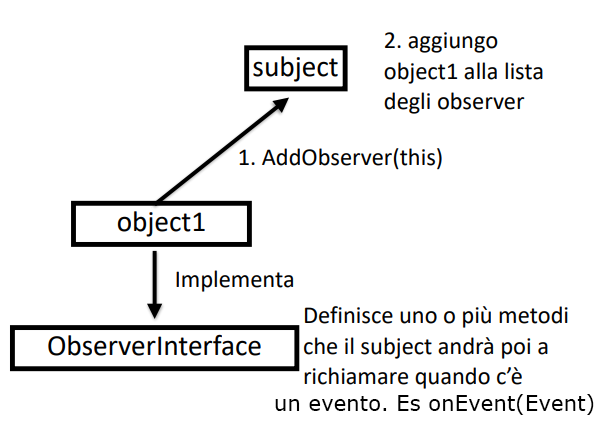
\includegraphics[width=.8\textwidth]{images/Mobile computing/6. Progettazione/observer registrazione.PNG}}
    \caption{Registrazione}
    \label{fig:registrazione}
\end{subfigure}\hfill
\quad
\begin{subfigure}[h]{0.5\textwidth}
    \centering
    \fbox{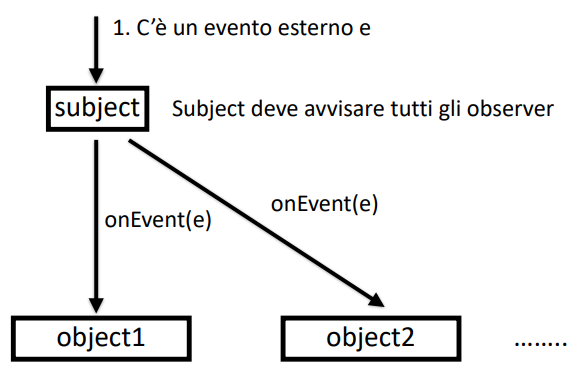
\includegraphics[width=.8\textwidth]{images/Mobile computing/6. Progettazione/observer notifica.PNG}}
    \caption{Notifica}
    \label{fig:notifica}
\end{subfigure}\hfill
\caption{Il pattern observer}
\end{figure}

Il pattern observer si può implementare con tanti observer o con un solo observer. 

Un modo per implementare il pattern observer con MVC è rappresentato in figura \ref{fig:pattern observer e MVC} 
Il controller si registra come observer con la view e la view si registra come observer con il model. Richiamami quando noti un evento.
\begin{figure}[!ht]
    \centering
    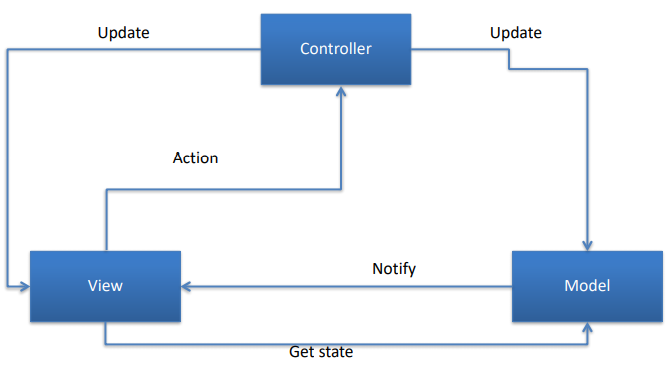
\includegraphics[width=.8\textwidth]{images/Mobile computing/6. Progettazione/observer e MVC.PNG}
    \caption{Pattern observer e MVC}
    \label{fig:pattern observer e MVC}
\end{figure}

\subsection{Vantaggi e svantaggi di MVC}
MVC è uno strumento molto utile per guidare la progettazione, ci aiuta a strutturare il codice in modo tale che possiamo trovare la struttura in ogni applicazione. 
Migliora il codice a livello di: 
\begin{itemize}
    \item leggibilità
    \item riusabilità
    \item mantenibilità
    \item testabilità
\end{itemize}

MVC ha dei limiti: non sempre si riesce ad avere una separazione netta tra le tre componenti.
\\ Sia in Android che in iOS si usano delle componenti combinate di MVC, componenti che mostrano l'informazione all'utente e gestiscono gli eventi:
\begin{itemize}
    \item ViewController in iOS
    \item Activity in Android
\end{itemize}

MVC non si adatta a soluzioni complesse come ad esempio una situazione in cui ci sono più schermate. 
L'idea è quella di avere un controller generale (detto coordinating controller) per l'applicazione e vari view-controller (detti mediating controller) per le singole schermate. 

\begin{figure}[!ht]
    \centering
    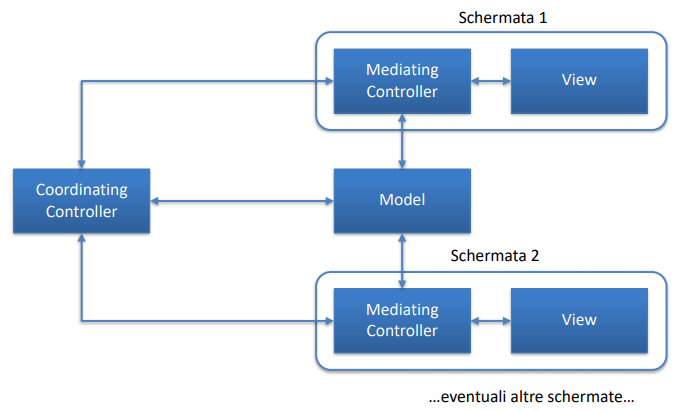
\includegraphics[width=.8\textwidth]{images/Mobile computing/6. Progettazione/mediating controller.PNG}
    \caption{Mediating controller}
    \label{fig:mediating controller}
\end{figure}

Uno dei principali motivi dell'utilizzo del MVC è la riusabilità del model. Idealmente il model può essere utilizzato sia da applicazioni per dispositivi mobili che per dispositivi tradizionali. 

Le classi del Model sono riutilizzabili tra applicazioni che condividono le stesse strutture dati, ad esempio in Java il Collection Framework. 

Gli oggetti View sono riutilizzabili tra tutte le applicazioni che 
condividono gli stessi strumenti di interfaccia, anche se le funzionalità delle applicazioni sono completamente diverse.

Il Controller è il più complicato da riutilizzare, è specifico all'app e alla piattaforma e difficilmente può essere condiviso tra client e server o tra due applicazioni diverse.
Anche se il controller è più difficilmente riutilizzabile, esistono alcuni problemi comuni che sono indipendenti dalle applicazioni.
Esistono delle classi definite nei framework per risolvere questi problemi.

Gli strumenti di sviluppo per applicazioni mobili sono pensati per uno sviluppo basato su MVC.
Gli ambienti di sviluppo permettono di creare in modo statico gli elementi di View. 
Permettono anche di creare il legame tra view e controller. 
